\chapter{Progettazione}

\textit{In questo capitolo vengono presentate le scelte progettuali definite a monte della stesura del codice:
l'architettura del sistema, i protocolli di comunicazione e i formati dati adottati, nonché i pattern architetturali
scelti per la loro realizzazione. La descrizione ha lo scopo di motivare tali decisioni, rimandando al capitolo
successivo la loro effettiva traduzione in codice.}

\section{Situazione di partenza} \label{sec:situazione-partenza}

Questa sezione descrive l'architettura del firmware così come si presentava prima dell'inizio del tirocinio, allo scopo di fornire un punto
di riferimento rispetto a cui distinguere, nelle sezioni successive, i contributi introdotti durante il lavoro svolto.

\subsection{Architettura}

Il firmware implementava un meccanismo di acquisizione e persistenza dei dati, basato sulla suddivisione in \textbf{producer}, uno per
sensore, e un unico \textbf{consumer} dedicato alla scrittura su microSD. I due ruoli comunicavano tramite una coda di richieste di scrittura,
ciascuna costituita da un riferimento al buffer dati da trascrivere, dalla sua lunghezza e dall'identificativo del sensore che lo ha prodotto.\\
All'accensione, ottenuta semplicemente collegando il dispositivo a una fonte di alimentazione, il firmware avviava automaticamente l'acquisizione 
dei dati, senza richiedere alcun comando esplicito da parte dell'utente. La persistenza avveniva affidandosi al file system \gls{fat}: ciascun blocco
di dati (\emph{chunk}) veniva salvato come file separato in formato \textbf{CSV}.\\
Per evitare che la scrittura su microSD bloccasse l'acquisizione dati, a ogni producer erano associati due buffer alternati:
mentre uno veniva scritto su microSD dal consumer, l'altro restava disponibile per contenere i dati recuperati dai sensori. Tali
ruoli possono scambiarsi durante l'esecuzione normale del firmware. \\
Indipendentemente dal meccanismo di persistenza, il firmware trasmetteva già i dati acquisiti in tempo reale all'app EggLog tramite BLE,
permettendo la visualizzazione \textit{live} delle grandezze rilevate durante la sessione, in parallelo alla loro scrittura su microSD.

\begin{figure}[H]
    \centering
    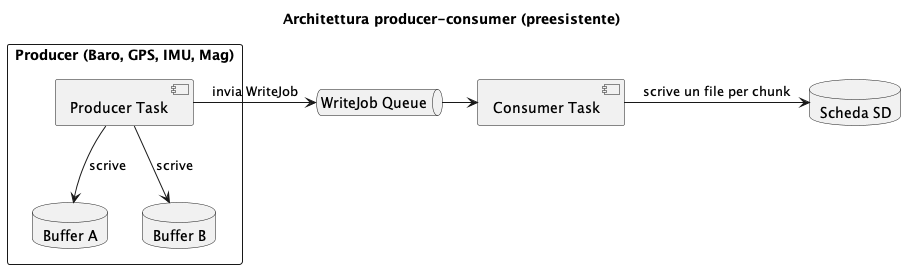
\includegraphics[width=\textwidth]{../img/puml/diagrammi/producer-consumer.png}
    \caption{Architettura producer-consumer preesistente}
\end{figure}

\subsection{Scelte progettuali}

\begin{itemize}
    \item \textbf{Producer-Consumer}: separazione netta tra il ruolo di acquisizione dati e quello di persistenza, disaccoppiati tramite una coda di richieste di scrittura.
    \item \textbf{Double buffering (ping-pong buffer)}: permette lettura e scrittura concorrenti sullo stesso flusso di dati senza reciproco blocco.
    \item \textbf{Container singleton per la configurazione}: la configurazione è esposta tramite due punti di accesso globali unici, che incapsulano l'accesso concorrente
    allo stato condiviso. I parametri di configurazione persistenti sono memorizzati in memoria non volatile, garantendone la conservazione anche dopo
    il riavvio del dispositivo.
    \item \textbf{Trasmissione dati in tempo reale via BLE}: il flusso di dati verso l'app è disaccoppiato dal meccanismo di persistenza su microSD, 
    permettendo la visualizzazione live delle grandezze rilevate senza dipendere dalla scrittura effettiva dei dati su file.
\end{itemize}

Queste scelte erano già consolidate nella base di codice ricevuta all'inizio del tirocinio e sono state mantenute come fondamenta su cui innestare gli
interventi successivi, descritti nelle sezioni seguenti.

\newpage



Le sezioni che seguono descrivono in dettaglio le scelte progettuali introdotte nel corso del tirocinio, organizzate secondo le seguenti aree funzionali:
\begin{itemize}
    \item persistenza dei dati su microSD;
    \item gestione dello stato globale del dispositivo;
    \item segnalazione visiva tramite LED;
    \item gestione dell'inattività dei sensori;
    \item gestione della sessione di acquisizione;
    \item gestione della calibrazione dell'altitudine;
    \item gestione della calibrazione dell'IMU;
    \item valutazione tecnica dello sniffer CAN e della sua architettura.
\end{itemize}

Per inquadrare l'architettura del sistema prima di entrarne nel dettaglio, le figure seguenti adottano la notazione del modello C4, che descrive un sistema 
attraverso viste innestate a livello di dettaglio crescente. La Figura \ref{fig:c4-context} presenta una vista di contesto, posizionando il dispositivo EggLog 
rispetto agli attori e ai sistemi esterni con cui interagisce: il pilota, EggLog App, il bus CAN del motoveicolo e EggLog CAN Sniffer. \\
La Figura \ref{fig:c4-container} ne approfondisce la struttura interna a livello di container, distinguendo il firmware in esecuzione sul microcontrollore dalla 
persistenza su scheda microSD.\\
A partire da questo inquadramento generale, valido per l'intero capitolo, ciascun gruppo di sezioni successive è introdotto da un diagramma dei componenti che 
mette a fuoco i soli moduli rilevanti per quell'area funzionale. Il primo, riportato in Figura \ref{fig:c4-persistenza}, riguarda la persistenza dei dati e la 
gestione dello stato condiviso, argomenti delle due sezioni immediatamente seguenti.

\begin{figure}[H]
    \centering
    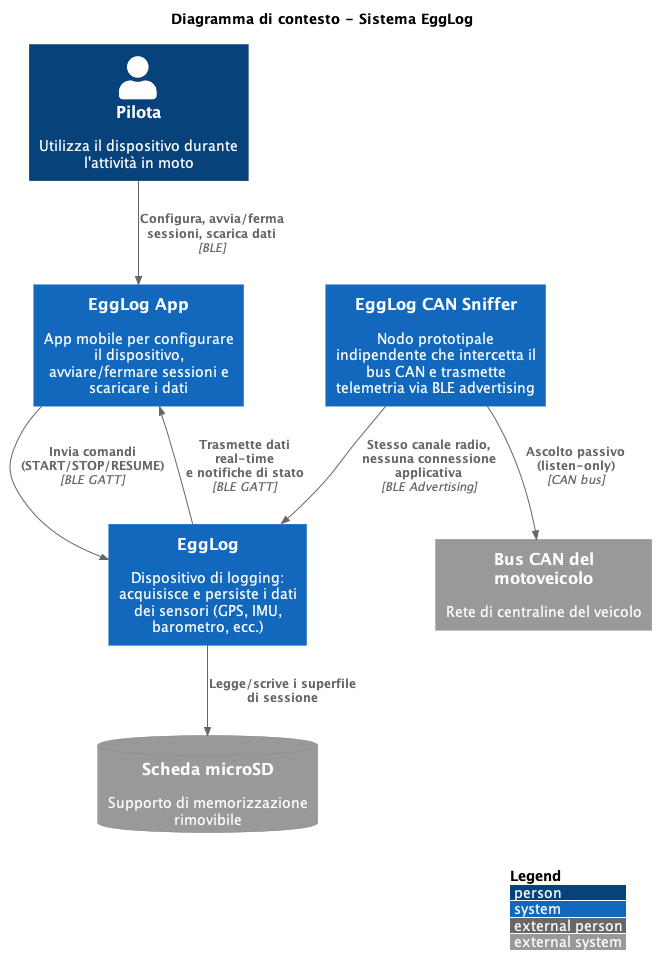
\includegraphics[width=0.8\textwidth]{../img/puml/c4/C4_Context_EggLog.png}
    \caption{Diagramma di contesto del sistema EggLog}
    \label{fig:c4-context}
\end{figure}

\begin{figure}[H]
    \centering
    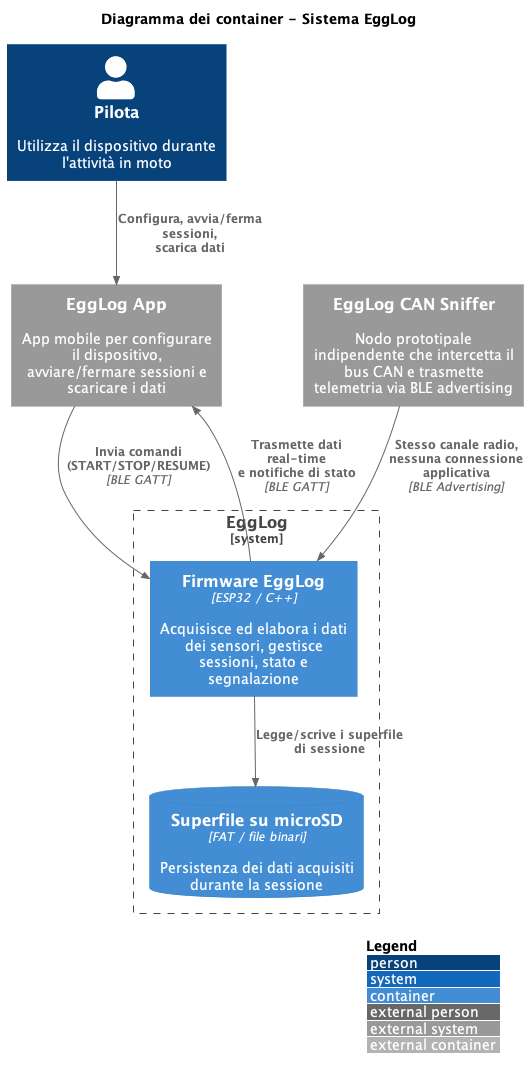
\includegraphics[width=0.7\textwidth]{../img/puml/c4/C4_Container_EggLog.png}
    \caption{Diagramma dei container del sistema EggLog}
    \label{fig:c4-container}
\end{figure}

\begin{figure}[H]
    \centering
    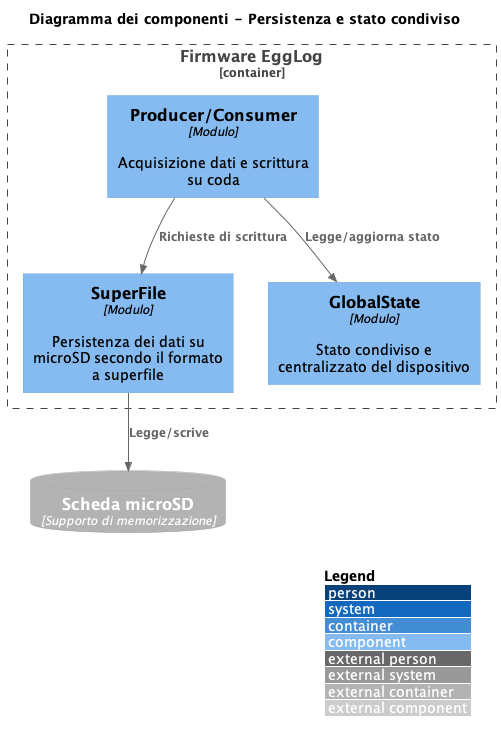
\includegraphics[width=0.6\textwidth]{../img/puml/c4/C4_Component_EggLog_Persistenza.png}
    \caption{Diagramma dei componenti del firmware EggLog: persistenza e stato condiviso}
    \label{fig:c4-persistenza}
\end{figure}

\section{Sistema di persistenza a superfile} \label{sec:superfile}

\subsection{Architettura}

Il layer di persistenza a basso livello viene progettato come un modulo concettualmente diviso in due responsabilità nettamente separate:

\begin{itemize}
    \item \textbf{formato su disco}, ovvero l'insieme minimo di informazioni che devono essere scritte fisicamente all'inizio del file
    affinché esso sia autodescrittivo e riapribile in modo corretto anche dopo un riavvio del dispositivo;
    \item \textbf{stato di runtime}, ovvero l'insieme di informazioni necessarie a operare sul file mentre il dispositivo è acceso. Tali informazioni possono essere: 
    il riferimento al file aperto, i parametri derivati dal sensore associato, la dimensione del \gls{record} (che varia da sensore a sensore), la capacità e 
    soglie operative.
\end{itemize}

Le operazioni concettuali che il modulo mette a disposizione sono: creazione di un nuovo file, apertura con eventuale recupero dello stato dopo
un'interruzione imprevista, scrittura di un blocco di record, sincronizzazione periodica dell'header su disco e in fine chiusura. Tali operazioni sono pensate
come funzioni indipendenti che agiscono su un'istanza esplicita del file, anziché come comportamento implicito legato a uno stato nascosto: questa
scelta è motivata dalla volontà di restare aderenti a uno stile a basso \textit{overhead}, coerente con i vincoli di un sistema embedded a risorse limitate.

Il modulo non contiene alcuna logica di concorrenza al proprio interno: l'accesso concorrente da parte di più sensori è delegato interamente al layer
superiore (il consumer già presente nella base di codice preesistente), che invoca le operazioni sotto un lock esplicito sul canale di comunicazione
condiviso con la scheda microSD.

Si mantiene così una separazione netta di responsabilità tra:
\begin{itemize}
    \item cosa scrivere e come è organizzato il file;
    \item quando scrivere e con quali garanzie di sincronizzazione tra le diverse fonti di dati.
\end{itemize}

\subsection{Scelte progettuali}

\begin{itemize}
    \item \textbf{Separazione tra formato persistito e stato operativo}: il layout dei dati salvati su disco è pensato come concettualmente indipendente
    dallo stato necessario per operare sul file durante l'esecuzione.\\
    \textit{Vantaggio}: un'evoluzione futura del formato su disco (ad esempio un nuovo
    campo nell'header) non richiede di intervenire sulla logica di gestione del file, e viceversa; la presenza di un identificativo di versione nell'header
    rende inoltre possibile, in linea di principio, gestire in futuro più versioni di formato senza rompere la compatibilità con i file già scritti.

    \item \textbf{Finestra di azzeramento anticipata (\emph{pre-zeroed lookahead window})}: illustrata in dettaglio nella sezione dedicata alla recovery
    (\hyperref[subsec:Recovery]{Recovery dopo interruzioni impreviste}). \\
    \textit{Vantaggio}: permette una recovery deterministica dopo un'interruzione imprevista, a fronte di un costo aggiuntivo di scrittura minimo.
\end{itemize}

\subsection{Formato su disco: l'header}

Ogni superfile è organizzato in due aree contigue: un'\textbf{area di intestazione} (header), di dimensione fissa e allineata al settore fisico
del supporto di memorizzazione, seguita da un'\textbf{area dati}, costituita da una sequenza di record a dimensione fissa specifica per ciascun sensore.

L'header è l'unica porzione di stato che viene effettivamente persistita sul supporto e che descrive il contenuto del file: deve quindi contenere
tutte le informazioni necessarie a riaprire correttamente il file dopo un riavvio del dispositivo, senza dover rileggere per intero l'area dati.
Dal punto di vista concettuale, l'header è composto dai seguenti campi logici:

\begin{itemize}
    \item \textbf{Versione del formato}: identifica la revisione del layout con cui il file è stato scritto, per consentire in futuro l'evoluzione
    del formato mantenendo la compatibilità con i file già esistenti;
    \item \textbf{Identificativo del sensore}: associa in modo univoco il file al sensore che lo ha prodotto;
    \item \textbf{Dimensione del record}: numero di byte occupati da ciascun record, specifico per il tipo di sensore;
    \item \textbf{Capacità totale}: numero massimo di record che il file può contenere, calcolato una sola volta alla creazione del file 
    (approfondita in \hyperref[subsec:capacita_superfile]{Capacità del file});
    \item \textbf{Cursore di fine dati}: posizione, all'interno dell'area dati, del primo record ancora libero, cioè il punto in cui avverrà la
    prossima scrittura;
    \item \textbf{Cursore di inizio dati}: posizione del più vecchio record ancora considerato valido; rilevante unicamente per i sensori che
    operano in modalità a sovrascrittura;
    \item \textbf{Soglia di sincronizzazione}: intervallo, espresso in numero di record scritti, dopo il quale l'header viene ripersistito su disco
    (approfondito in \hyperref[subsec:sincronizzazione_header]{Sincronizzazione header});
    \item \textbf{Dimensione della finestra di azzeramento}: numero di record, immediatamente successivi al cursore di fine dati, mantenuti
    costantemente pre-azzerati (approfondito in \hyperref[subsec:fin_azzeramento]{Finestra di azzeramento});
    \item \textbf{Indicatori di stato}: informazioni booleane quali l'abilitazione della modalità a sovrascrittura o il raggiungimento della
    capacità massima del file.
\end{itemize}

La figura seguente riassume questi campi logici e la loro collocazione all'interno del file.

\begin{figure}[H]
    \centering
    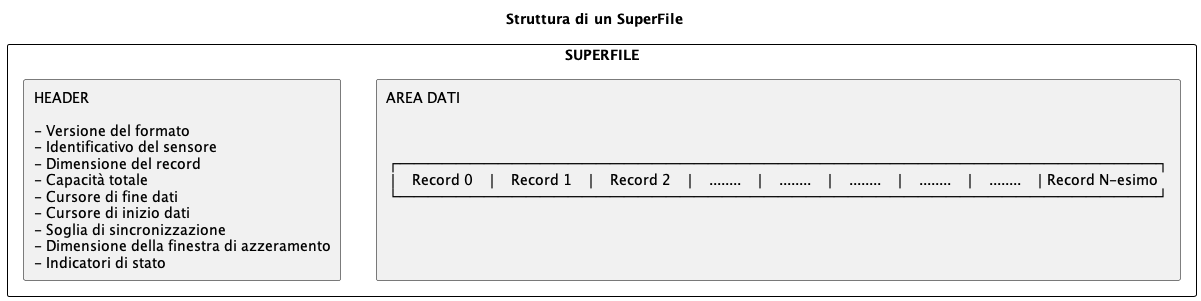
\includegraphics[width=0.95\textwidth]{../img/puml/diagrammi/superfile_layout.png}
    \caption{Campi logici dell'header del superfile}
\end{figure}

\subsection{Capacità del file} \label{subsec:capacita_superfile}

La capacità totale del file, in numero di record, viene calcolata una sola volta al momento della creazione, a partire dall'\gls{odr} del sensore, 
dalla dimensione del suo record e dalla finestra temporale di conservazione dei dati desiderata (\emph{retention}).
Il valore ottenuto viene arrotondato per eccesso in modo da allinearsi alle unità di allocazione del supporto di memorizzazione, così da garantire
che il file, una volta preallocato per intero, occupi esclusivamente spazio contiguo, evitando la frammentazione che affliggeva la soluzione a
file multipli descritta nella \hyperref[sec:situazione-partenza]{Situazione di partenza}.

\subsection{Scrittura e \textit{wraparound}}

L'area dati del superfile è concettualmente organizzata come un \textbf{buffer circolare}: la scrittura di un nuovo blocco di record calcola la
posizione di partenza a partire dal cursore di fine dati corrente e verifica se il blocco attraversa il limite superiore dell'area dati; in tal caso
l'operazione viene concettualmente spezzata in due scritture separate (\emph{pre-wrap} e \emph{post-wrap}), la seconda delle quali riparte dall'inizio
dell'area dati.

Per i sensori in modalità a sovrascrittura, il cursore di inizio dati avanza automaticamente quando il buffer si riempie, sacrificando
i record più vecchi. Per il sensore GPS, per il quale la sovrascrittura è disabilitata in quanto ritenuto una sorgente di dati più importante, 
al raggiungimento della capacità massima le scritture successive vengono ignorate e il file viene marcato come pieno, propedeuticamente alla
terminazione automatica della sessione.

\subsection{Sincronizzazione dell'header} \label{subsec:sincronizzazione_header}

Per limitare l'usura del supporto di memorizzazione e massimizzare il \textit{throughput} di scrittura, l'header non viene sincronizzato su disco 
a ogni singolo record scritto, ma periodicamente, al raggiungimento della soglia di sincronizzazione descritta in precedenza. Tale soglia non è un 
valore fisso comune a tutti i sensori, ma viene ricavata a partire da un budget di byte target da sincronizzare, rapportato alla dimensione del 
record del sensore. In questo modo, la frequenza di sincronizzazione risulta proporzionata al volume di dati effettivamente prodotto, indipendentemente 
dalla dimensione del singolo record.

Questa scelta introduce tuttavia un problema di consistenza in caso di arresto imprevisto del dispositivo. Tra due sincronizzazioni dell'header, 
infatti, possono essere già presenti sul supporto record scritti successivamente all'ultimo aggiornamento dell'header, dei quali quest'ultimo non è 
ancora a conoscenza. È quindi necessario disporre di un meccanismo che permetta di individuare e recuperare correttamente tali record durante la 
successiva apertura del file. Tale meccanismo è descritto nella sezione immediatamente successiva
(\hyperref[subsec:fin_azzeramento]{Finestra di azzeramento}).

\begin{figure}[H]
    \centering
    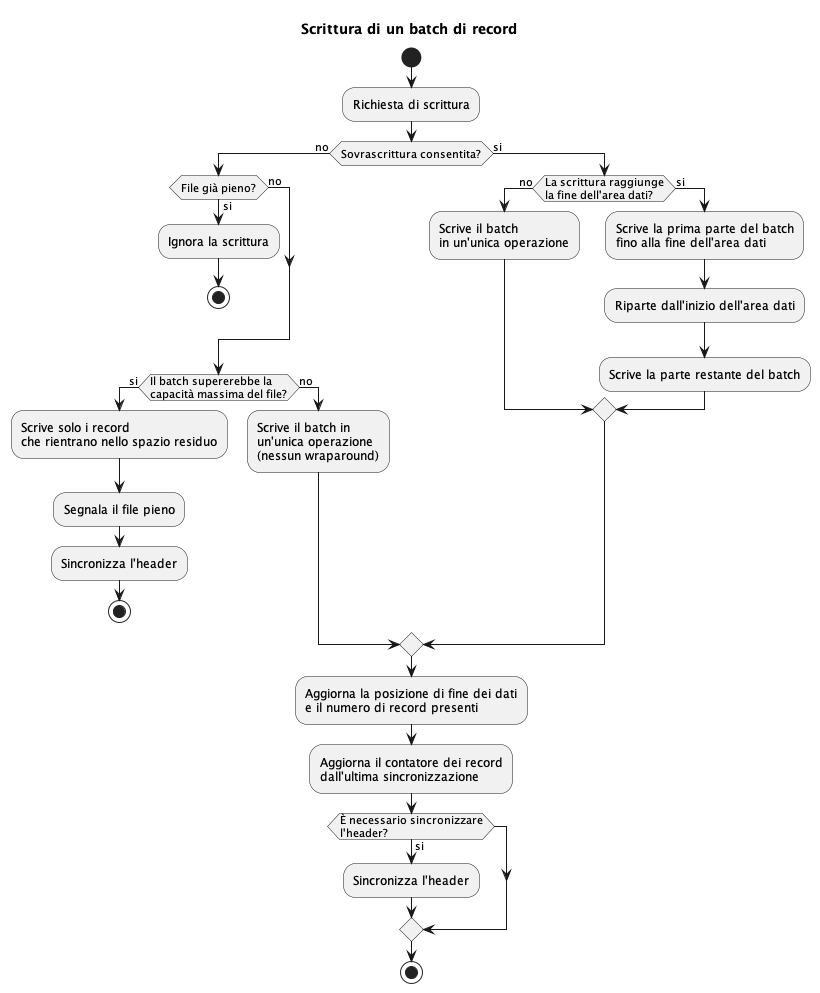
\includegraphics[width=0.9\textwidth]{../img/puml/diagrammi/superfile_write.png}
    \caption{Diagramma di flusso della scrittura di un insieme di record}
\end{figure}

\subsection{Finestra di azzeramento} \label{subsec:fin_azzeramento}

A supporto della procedura di recovery viene mantenuta una \textbf{finestra di record pre-azzerati} immediatamente davanti al cursore di scrittura. 
La finestra ha una dimensione pari a un multiplo della soglia di sincronizzazione ed è costituita da record inizializzati a zero. Poiché ogni record 
valido inizia con un marcatore temporale non nullo, un record contenente esclusivamente valori azzerati può essere identificato come non ancora scritto.

La finestra viene inizializzata alla creazione del file e ricostituita a ogni sincronizzazione dell'header, subito dopo l'avanzamento del cursore di 
scrittura. In caso di arresto imprevisto, la presenza dei record pre-azzerati permette quindi di delimitare l'area potenzialmente contenente dati non 
ancora riportati nell'header e di effettuare una recovery coerente dello stato del file.

\begin{figure}[H]
    \centering
    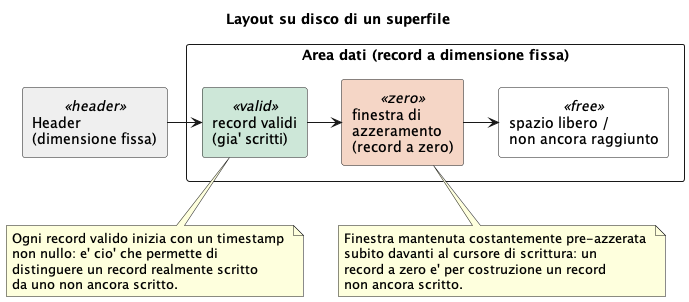
\includegraphics[width=0.8\textwidth]{../img/puml/diagrammi/superfile_disk_layout.png}
    \caption{Layout su disco del superfile: area dati valida, finestra di azzeramento e spazio libero}
\end{figure}

\subsection{Recovery dopo interruzioni impreviste} \label{subsec:Recovery}

Il meccanismo di recovery si appoggia, a livello di singolo superfile, proprio sulla finestra di azzeramento appena descritta.
All'apertura di un superfile in modalità recupero, l'header letto da disco può quindi non riflettere l'esatto stato dei dati realmente presenti: 
la procedura di riconciliazione scandisce in avanti, record per record,
a partire dalla posizione indicata dall'header, leggendo unicamente il marcatore temporale iniziale di ciascun record. Finché il marcatore letto è
diverso da zero, il record viene considerato realmente scritto e il cursore viene avanzato, con la stessa logica usata durante la scrittura normale;
la scansione si interrompe al primo marcatore nullo, che identifica in modo affidabile il vero confine tra dati validi e finestra pre-azzerata. Al
termine della riconciliazione, l'header aggiornato viene risincronizzato su disco e la finestra di azzeramento ricostituita a partire dalla nuova
posizione del cursore, ripristinando le condizioni necessarie per riprendere normalmente l'acquisizione.

A livello di dispositivo, l'intera procedura di recovery rimonta il file system, ricarica la configurazione persistita e, solo se lo stato globale
indica una sessione di logging in corso, recupera il riferimento alla sessione attiva e richiama la riconciliazione per tutti i superfile della
sessione; un fallimento in una qualsiasi di queste fasi imposta lo stato di errore globale, mentre il successo lo azzera esplicitamente, permettendo
all'acquisizione di riprendere da dove si era interrotta, senza perdita né duplicazione dei dati già scritti.

\begin{figure}[H]
    \centering
    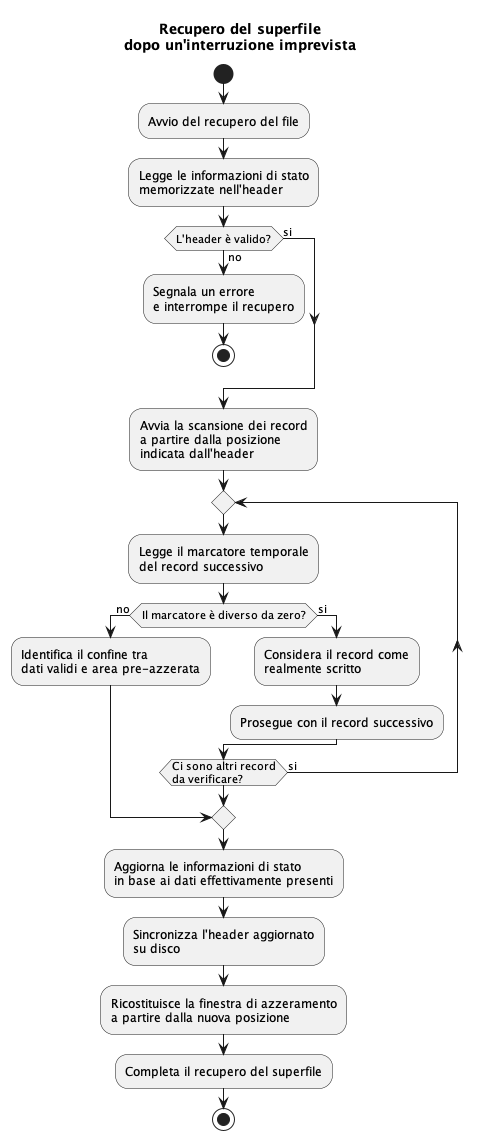
\includegraphics[width=0.6\textwidth]{../img/puml/diagrammi/superfile_recovery.png}
    \caption{Flusso di recovery di un superfile dopo un'interruzione imprevista}
\end{figure}

\newpage

\section{Stato globale del dispositivo}

\subsection{Architettura}

Lo stato globale del dispositivo rappresenta il punto di accesso centralizzato allo stato operativo, condiviso in lettura e scrittura da un numero
elevato di componenti indipendenti: la gestione della sessione, la segnalazione mediante LED, la gestione dell'inattività, lo stato della microSD, la
calibrazione dell'IMU, il modulo di comunicazione BLE e tutti i task producer/consumer.

Concettualmente espone un insieme di indicatori booleani indipendenti: supporto di memorizzazione mancante, condizione di errore, calibrazione in corso,
sospensione per inattività, \textit{pairing} in corso e download/cancellazione in corso, insieme a uno stato principale di sessione, con un numero
finito di valori: STAND\_BY, LOGGING, SUSPENDED, DOWNLOADING e DELETING. Ciascun indicatore è accessibile esclusivamente tramite un'interfaccia dedicata
di lettura e scrittura.

Il modulo era già presente, in forma preliminare, nella base di codice ricevuta all'inizio del tirocinio. Tuttavia, l'implementazione originale gestiva solo 
un sottoinsieme degli stati e non veniva utilizzata in tutte le transizioni previste dal codice. È stato pertanto completamente riprogettato e reimplementato 
nell'ambito del lavoro svolto durante il tirocinio.

\subsection{Scelte progettuali}

\begin{itemize}
    \item \textbf{Facade su stato condiviso atomico}: ogni variabile di stato è rappresentata come un'unità atomica ed è accessibile esclusivamente attraverso 
    un'interfaccia uniforme di lettura e scrittura. \\
    \textit{Vantaggio}: consente di gestire in modo sicuro gli accessi concorrenti ai singoli indicatori senza ricorrere a meccanismi di mutua esclusione, poiché 
    le operazioni di lettura e scrittura sono atomiche e indipendenti tra loro. Ciò riduce l'overhead associato all'utilizzo di mutex e limita il rischio di contesa
     tra i componenti che accedono allo stato condiviso.
    \item \textbf{Single Source of Truth}: nessun componente mantiene una propria copia locale dello stato del dispositivo; ogni decisione (ad esempio
    se il LED deve lampeggiare rosso, se un nuovo comando è accettabile, se sospendere i sensori) viene presa interrogando direttamente lo stato
    globale. \\
    \textit{Vantaggio}: evita disallineamenti tra componenti diversi che, in una versione precedente basata su variabili locali duplicate,
    potevano restare temporaneamente in stati incoerenti tra loro.
\end{itemize}

\newpage
Analogamente, la Figura \ref{fig:c4-segnalazione} restringe il campo ai soli moduli coinvolti nella segnalazione di stato e nel monitoraggio dei sensori, argomenti delle due 
sezioni immediatamente seguenti: la segnalazione tramite LED e la gestione dell'inattività dei sensori.

\begin{figure}[H]
    \centering
    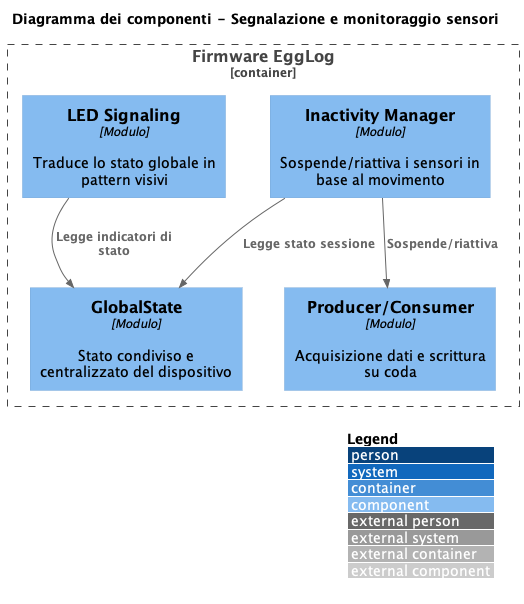
\includegraphics[width=0.6\textwidth]{../img/puml/c4/C4_Component_EggLog_Segnalazione.png}
    \caption{Diagramma dei componenti del firmware EggLog: segnalazione e monitoraggio sensori}
    \label{fig:c4-segnalazione}
\end{figure}

\section{Segnalazione di stato tramite LED}

\subsection{Architettura}

Il sottosistema di segnalazione LED è organizzato concettualmente in tre responsabilità nettamente separate
\begin{itemize}
    \item \textbf{Livello hardware}: incapsula esclusivamente il pilotaggio fisico del LED, isolando il resto del sistema dai dettagli dell'hardware.
    \item \textbf{Livello decisionale}: interroga lo stato globale del dispositivo e determina il pattern visivo da mostrare, senza accedere direttamente all'hardware.
    \item \textbf{Livello di rendering}: esegue un ciclo periodico, richiama il livello decisionale e traduce il pattern restituito in un'animazione effettiva, gestendo 
    la temporizzazione, il lampeggio e la dissolvenza.
\end{itemize}

\subsection{Scelte progettuali}

\begin{itemize}
    \item \textbf{Risoluzione a priorità esplicita}: il livello di decisione valuta lo stato del dispositivo
    secondo un ordine di priorità fisso ed esplicito (Tabella~\ref{tab:led-priorita}):
    \begin{table}[H]
        \centering
        \begin{tabular}{c l l l}
            \hline
            \textbf{Priorità} & \textbf{Stato} & \textbf{Colore} & \textbf{Animazione} \\
            \hline
            1 & MicroSD mancante & Rosso & Lampeggio rapido \\
            2 & Errore & Rosso & Lampeggio lento \\
            3 & Pairing BLE & Blu & Lampeggio \\
            4 & Pairing Wi-Fi & Blu & Lampeggio veloce \\
            5 & Calibrazione attiva & Giallo & Dissolvenza \\
            6 & Recupero dati durante la calibrazione & Giallo & Luce fissa \\
            7 & Download / cancellazione & Viola & Lampeggio \\
            8 & Sospensione & Verde & Dissolvenza lenta \\
            9 & Logging & Verde & Luce fissa \\
            10 & Standby & Bianco & Luce fissa \\
            \hline
        \end{tabular}
        \caption{Priorità e segnalazioni visive del sottosistema LED}
        \label{tab:led-priorita}
    \end{table}
    \textit{Vantaggio}: garantisce che, in presenza di più condizioni vere contemporaneamente (ad esempio, microSD mancante durante il logging), l'utente 
    veda sempre l'informazione più critica, invece di un comportamento indefinito o di un LED che cambia in modo instabile tra più stati concorrenti.
    \item \textbf{Value Object per il pattern visivo}: il pattern da visualizzare è rappresentato come un dato immutabile che descrive le caratteristiche 
    dell'animazione, quali colore, modalità di animazione e frequenza. Questa rappresentazione è mantenuta separata sia dalla logica che determina il pattern 
    da mostrare sia dal componente responsabile della sua effettiva visualizzazione.
    \textit{Vantaggio}: rende il livello di decisione verificabile in isolamento e disaccoppia completamente la logica di business dal dettaglio di rendering.
\end{itemize}

\newpage

\section{Gestione dell'inattività dei sensori}

\subsection{Architettura}

Il meccanismo di gestione dell'inattività implementa la sospensione automatica dei sensori non essenziali dopo un periodo di
inattività configurabile, e la loro riattivazione al rilevamento di movimento. La sorgente di riferimento primaria per il rilevamento del movimento
è il GPS, mentre l'accelerometro dell'IMU viene utilizzato come sorgente di \textbf{fallback}, attiva solo quando
il GPS non è considerato affidabile in quel momento. Tipicamente in assenza di un \gls{fixgnss} valido o recente come accadrebbe in ambienti con scarsa 
visibilità satellitare, come gallerie o zone urbane dense.
\subsection{Scelte progettuali}

\begin{itemize}
    \item \textbf{Strategy con sorgente autorevole commutabile}: una funzione di decisione
    determina, in base alla freschezza dell'ultimo fix GPS ricevuto, quale delle due sorgenti
    (GPS o IMU) debba governare la decisione di sospensione. Il percorso di rilevamento basato
    su IMU rimane sempre attivo, ma il suo risultato viene ignorato quando il GPS è considerato
    affidabile.\\
    \textit{Vantaggio}: i due percorsi di rilevamento rimangono indipendenti, mentre la
    selezione della sorgente autorevole è centralizzata in un unico punto di decisione,
    rendendo la logica più semplice da verificare e modificare.

    \item \textbf{\gls{debounce} basato su campioni consecutivi}: il rilevamento del
    movimento tramite GPS viene considerato valido solo dopo aver ricevuto un numero minimo
    di campioni consecutivi al di sopra della soglia prevista. Il conteggio viene azzerato
    quando viene rilevato un campione al di sotto della soglia.\\
    \textit{Vantaggio}: evita che singole misure anomale, dovute al rumore del segnale o agli
    effetti di \gls{multipath}, in particolare in ambiente urbano, provochino riattivazioni
    spurie dei sensori sospesi.

    \item \textbf{Sospensione esclude il GPS}: la sospensione e la riattivazione, propagate
    a tutti i task producer, escludono esplicitamente il GPS.\\
    \textit{Vantaggio}: il GPS rimane attivo durante la sospensione degli altri sensori,
    permettendo sia di rilevare autonomamente l'eventuale ripresa del movimento, sia di
    mantenere il fix già acquisito. Alla riattivazione degli altri sensori non è quindi
    necessario attendere una nuova acquisizione del fix, riducendo il buco di dati tra la
    sospensione e la ripresa della registrazione completa.
\end{itemize}

\subsection{Configurazione e comportamento ai bordi}

Il timeout di inattività è configurabile dall'utente tramite l'app tra i valori "mai", 10, 30 o 60 minuti; il valore "mai"
disabilita completamente la logica di sospensione, mantenendo i sensori sempre attivi indipendentemente dal movimento rilevato.

\begin{figure}[H]
    \centering
    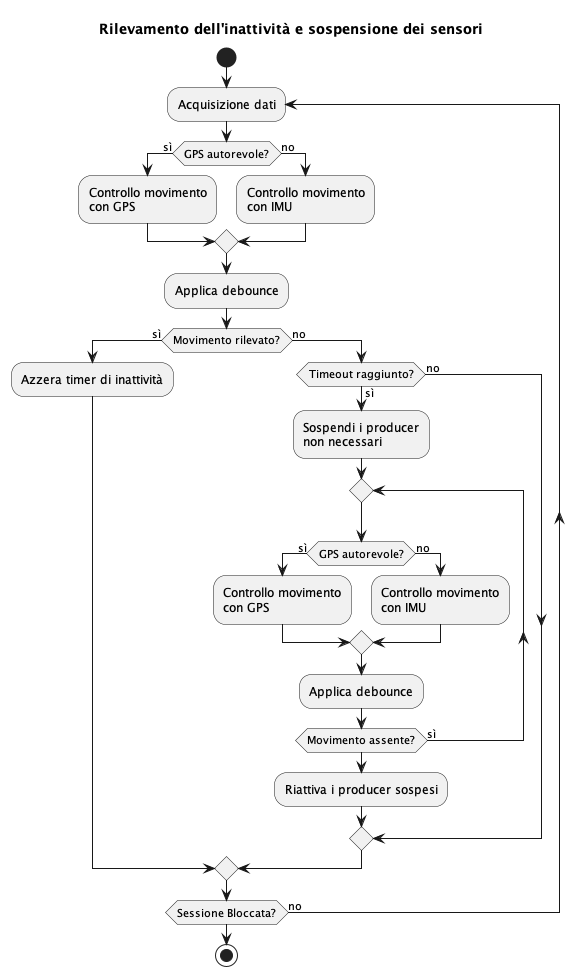
\includegraphics[width=0.7\textwidth]{../img/puml/diagrammi/inactivity_activity.png}
    \caption{Transizioni alla sospensione guidate da GPS con fallback IMU}
\end{figure}

\newpage

In modo analogo, la Figura \ref{fig:c4-sessione} mette a fuoco i moduli coinvolti nella gestione della sessione e nelle calibrazioni, argomenti 
delle tre sezioni seguenti: il protocollo di avvio e arresto della sessione, la calibrazione dell'altitudine e la calibrazione dell'IMU.

\begin{figure}[H]
    \centering
    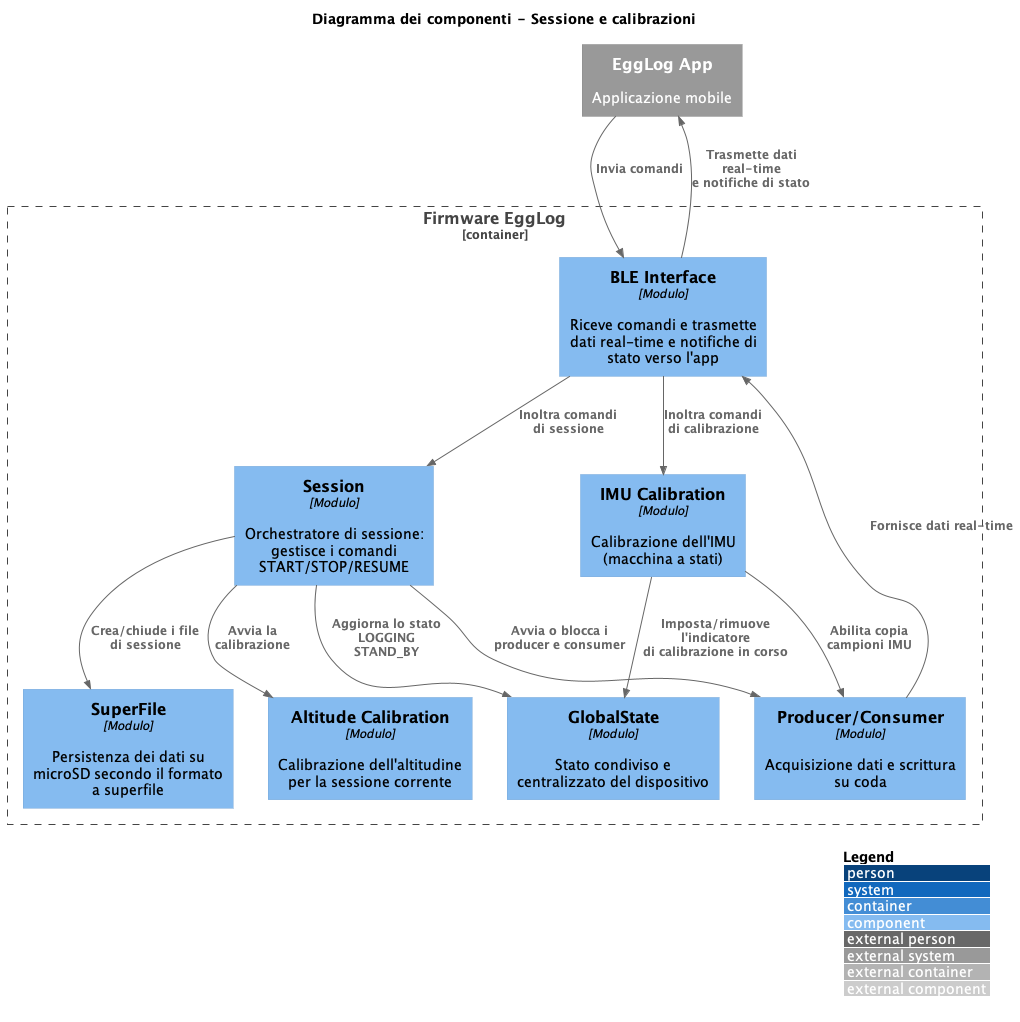
\includegraphics[width=1\textwidth]{../img/puml/c4/C4_Component_EggLog_Sessione.png}
    \caption{Diagramma dei componenti del firmware EggLog: sessione e calibrazioni}
    \label{fig:c4-sessione}
\end{figure}

\section{Protocollo di avvio e arresto della sessione}

\subsection{Architettura}

Il modulo di gestione della sessione si colloca come livello di orchestrazione sopra le componenti preesistenti: riceve i comandi dall'app tramite
BLE, coordina la creazione e la chiusura dei superfile (approfondito in \hyperref[sec:superfile]{superfile}), l'esecuzione della calibrazione dell'altitudine 
(approfondita in \hyperref[subsec:calibrazione_altitudine]{calibrazione altitudine}) e gli aggiornamenti dello stato globale del dispositivo, senza intervenire 
direttamente sulla logica interna di acquisizione dei singoli sensori.

\subsection{Scelte progettuali}

\begin{itemize}
    \item \textbf{Command Pattern}: i comandi provenienti dall'app (START, STOP, RESUME) sono rappresentati come valori distinti di un insieme
    chiuso, instradati da un unico punto di gestione, disaccoppiando totalmente l'esecuzione del comando dalla sua sorgente.\\
    \textit{Vantaggio}: la logica di sessione risulta verificabile e riutilizzabile anche da trigger diversi dal BLE, senza modifiche.
    \item \textbf{State Pattern}: le transizioni di stato del dispositivo (STAND\_BY, LOGGING, SUSPENDED, DOWNLOADING, DELETING) sono gestite
    centralmente dallo stato globale, e ogni decisione dipende esclusivamente dallo stato corrente.\\
    \textit{Vantaggio}: elimina condizionali diffusi nel codice che replicherebbero la stessa logica di stato in più punti, centralizzando le
    regole di transizione in un solo posto.
\end{itemize}

\subsection{Avvio sessione}

Alla ricezione del comando di avvio, se il dispositivo non è occupato in un'operazione di download o cancellazione e non è già in una sessione
attiva, il firmware esegue in sequenza:

\begin{enumerate}
    \item un tentativo di recovery della scheda microSD; in caso di fallimento, la sessione non viene avviata e viene notificato l'errore all'app;
    \item la generazione di un identificativo univoco di sessione, ottenuto combinando: l'identificativo del dispositivo, un riferimento temporale di
    inizio sessione e il marcatore \texttt{\_ACTIVE} che segnala la sessione come ancora in corso;
    \item la creazione del contenitore di sessione e dei relativi superfile per tutti i sensori;
    \item l'esecuzione sincrona della calibrazione dell'altitudine, il cui esito viene applicato immediatamente come riferimento di pressione per la 
    sessione;
    \item la scrittura di un insieme di metadati di sessione, contenente l'esito della calibrazione altitudine, il valore di pressione di
    riferimento ed eventuali condizioni di timeout;
    \item l'aggiornamento dello stato globale a LOGGING, la riattivazione forzata dei produttori di dati e l'avvio di una notifica periodica dello stato 
    di sessione verso l'app.
\end{enumerate}

Ogni fase è protetta da un accesso esclusivo al canale di comunicazione condiviso, con condizioni di timeout configurabili: in caso di mancata
acquisizione dell'accesso esclusivo o di fallimento di una delle operazioni, il firmware imposta lo stato di errore e interrompe l'avvio,
notificando comunque lo stato aggiornato all'app.

\begin{figure}[H]
    \centering
    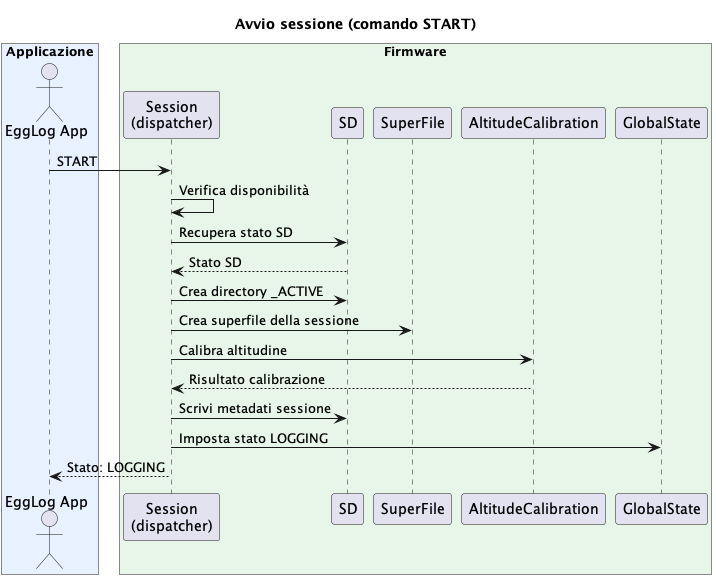
\includegraphics[width=0.85\textwidth]{../img/puml/diagrammi/Avvio-sessione.png}
    \caption{Diagramma di sequenza del comando START}
\end{figure}

\subsection{Arresto sessione}

Il comando di arresto (così come l'arresto automatico per esaurimento spazio GPS) innesca una sequenza di chiusura pensata per non
perdere dati residui nei buffer:

\begin{enumerate}
    \item se il dispositivo era in stato SUSPENDED, i produttori di dati vengono prima riattivati forzatamente;
    \item viene richiesto lo svuotamento sincrono di tutti i buffer dei sensori verso il meccanismo di scrittura, con timeout;
    \item il firmware attende che tutte le richieste di scrittura pendenti vengano completate;
    \item tutti i superfile della sessione vengono chiusi, sempre sotto accesso esclusivo al canale condiviso;
    \item il contenitore di sessione viene rinominato, sostituendo il marcatore \texttt{\_ACTIVE} con un riferimento temporale di fine sessione;
    \item lo stato torna a STAND\_BY e la notifica periodica viene interrotta.
\end{enumerate}

Un caso particolare è l'arresto automatico per esaurimento dello spazio dedicato al GPS: il firmware imposta un indicatore dedicato prima di
eseguire la stessa procedura di arresto, distinguendo per l'app un arresto voluto dall'utente da uno automatico.

\begin{figure}[H]
    \centering
    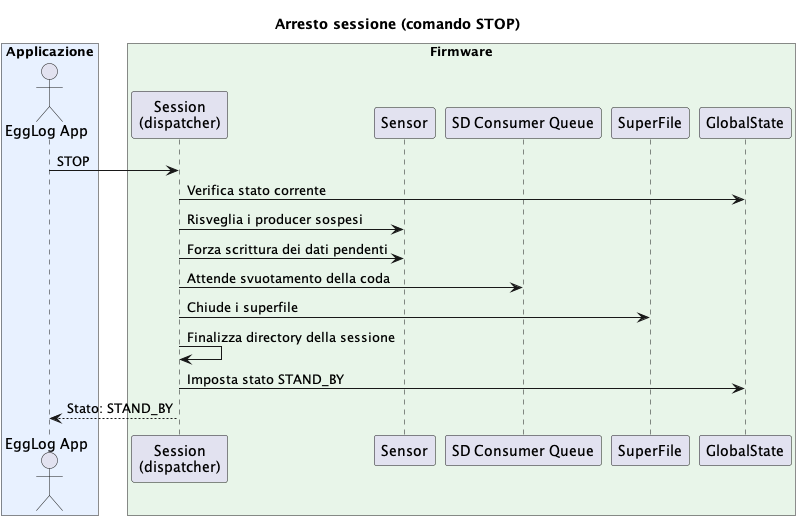
\includegraphics[width=\textwidth]{../img/puml/diagrammi/Arresto-sessione.png}
    \caption{Diagramma di sequenza del comando STOP}
\end{figure}

\newpage

\section{Calibrazione dell'altitudine} \label{subsec:calibrazione_altitudine}

\subsection{Architettura}

La calibrazione dell'altitudine è invocata in modo sincrono all'interno del flusso di avvio sessione, prima della transizione a LOGGING, e si basa
sull'ultima lettura disponibile del barometro, senza richiedere un canale dedicato di comunicazione con il relativo sensore.

\subsection{Algoritmo di calibrazione}

La calibrazione dell'altitudine garantisce che, se disponibile, il riferimento di pressione sia valido fin dal primo campione
registrato nella sessione. L'algoritmo raccoglie ripetutamente campioni di pressione, filtrando i duplicati tramite confronto del riferimento
temporale. Raggiunto un numero sufficiente di campioni, viene calcolata la \textbf{mediana} del gruppo (scelta più robusta della media rispetto a
campioni anomali) e la relativa \textbf{deviazione standard}: se questa è sotto una soglia prestabilita, il valore mediano viene accettato come
riferimento; altrimenti il gruppo viene scartato e la raccolta ricomincia. L'intera procedura è racchiusa in un timeout massimo, oltre il quale la
calibrazione è marcata come fallita e la sessione prosegue comunque, senza riferimento di altitudine valido.

A differenza della calibrazione IMU, valida per tutte le sessioni successive fino a nuova ricalibrazione, la calibrazione dell'altitudine è
\textbf{specifica di ogni singola sessione}: viene ripetuta a ogni avvio e persistita solo nei metadati della sessione corrente.

\begin{figure}[H]
    \centering
    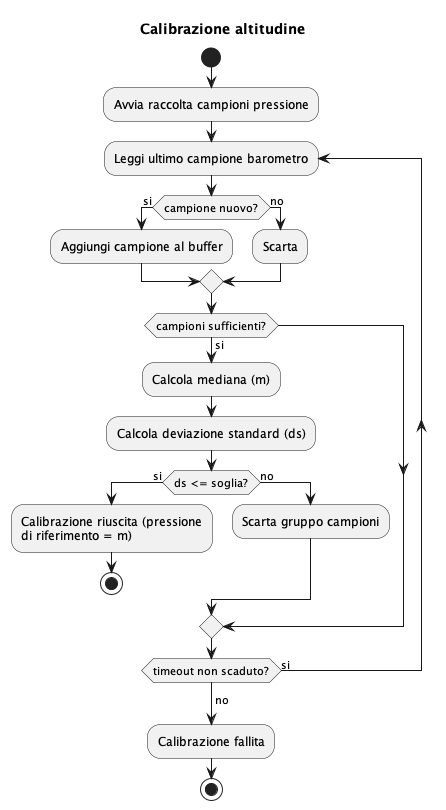
\includegraphics[width=0.6\textwidth]{../img/puml/diagrammi/Calibrazione-altitudine.png}
    \caption{Diagramma di flusso della calibrazione altitudine}
\end{figure}

\newpage

\section{Calibrazione dell'IMU}
Data l'importanza di questo modulo ai fini dell'accuratezza dei dati registrati, la progettazione della calibrazione dell'IMU è stata condotta con 
un livello di dettaglio maggiore rispetto agli altri componenti del sistema.

\subsection{Architettura}

La calibrazione dell'IMU è un'attività indipendente eseguibile esclusivamente nello stato \texttt{STAND\_BY}, quindi mai durante una sessione attiva o in 
presenza di un errore. All'avvio, viene risvegliato il task producer dell'IMU, che acquisisce normalmente i campioni di accelerometro e giroscopio. Quando 
la calibrazione è attiva, una variabile booleana ne abilita la copia in un \textbf{buffer dedicato}, separato dai due buffer utilizzati per il normale 
\textit{ping-pong buffering}. Il task di calibrazione consuma quindi questi campioni ed esegue le elaborazioni previste a ogni step, svuotando il buffer 
all'inizio di ciascuna fase per considerare esclusivamente i dati pertinenti.

La procedura è gestita tramite due distinti canali BLE: uno per i comandi inviati dall'app e uno per le notifiche con cui il firmware comunica in tempo 
reale lo stato della calibrazione.

\subsection{Scelte progettuali}

\begin{itemize}
    \item \textbf{State Pattern}: l'intera procedura è modellata come una macchina a stati esplicita (inattiva, pronta per lo step $n$, step $n$ in
    corso, step $n$ da ripetere, dati assenti, successo, errore), con un unico punto di gestione che interpreta il comando ricevuto in funzione dello
    stato corrente.\\
    \textit{Vantaggio}: ogni stato ammette solo un sottoinsieme ben definito di transizioni valide, evitando che comandi ricevuti
    fuori sequenza (ad esempio una conferma prima di un avvio) producano comportamenti indefiniti.

    \item \textbf{Command Pattern}: i comandi provenienti dall'app (avvio, conferma, interruzione) sono valori distinti di un insieme chiuso,
    instradati tramite una coda verso l'unico punto di gestione. \\
    \textit{Vantaggio}: la ricezione del comando è completamente disaccoppiata dalla
    sua esecuzione, evitando di eseguire logica di calibrazione potenzialmente bloccante direttamente nel contesto di ricezione BLE.
    \item \textbf{Fan-out non invasivo sul flusso dati}: l'acquisizione IMU continua a funzionare esattamente come se la calibrazione non esistesse,
    limitandosi a duplicare ogni campione anche verso il canale dedicato quando la calibrazione è attiva. \\
    \textit{Vantaggio}: la funzionalità di calibrazione è pensata come estensione additiva dell'acquisizione esistente, senza modificarne la logica interna 
    né rischiare di introdurre egressioni sul percorso dati principale.
    \item \textbf{Retry isolato per singolo step}: ogni fallimento per dati insufficienti riporta la macchina a uno stato di ripetizione specifico
    per lo step corrente, anziché allo stato d'errore. \\
    \textit{Vantaggio}: l'utente può ripetere solo lo step fallito, mantenendo il lavoro già validato negli step precedenti.
\end{itemize}

\subsubsection{Algoritmo di calibrazione}

Ogni step di misura si basa su un meccanismo comune di raccolta campioni, che integra tre elementi distinti:

\begin{itemize}
    \item un intervallo di \emph{assestamento} durante il quale i campioni ricevuti vengono scartati, per dare all'utente il tempo di portare il
    dispositivo nella posizione richiesta prima che la misura effettiva inizi;
    \item una raccolta a tempo, con calcolo incrementale di media e, dove richiesto, varianza del modulo dell'accelerazione;
    \item un meccanismo di \textbf{uscita anticipata}: superata una durata minima e un numero minimo di campioni, viene valutata la stabilità delle
    ultime letture; se il segnale risulta sufficientemente stabile, lo step termina prima dello scadere del timeout completo, riducendo i tempi di
    attesa percepiti dall'utente quando il dispositivo è già fermo nella posizione corretta.
\end{itemize}

\paragraph{Step 1 - Posizione dritta}
Con il dispositivo fermo vengono raccolti i campioni dell'IMU per verificarne la stabilità e la coerenza con l'accelerazione di gravità attesa. 
In caso di esito positivo, lo step determina l'asse verticale del sistema di riferimento e i bias di accelerometro e giroscopio da applicare 
nelle acquisizioni successive; in caso contrario, lo step viene rifiutato.

\paragraph{Step 2 - Inclinazione a destra}
Il dispositivo viene inclinato lateralmente rispetto al mezzo su cui è montato. Dallo scostamento rispetto alla posizione registrata nello step 
precedente viene derivato l'asse laterale del sistema di riferimento; un'inclinazione giudicata insufficiente comporta il rifiuto dello step.

\paragraph{Step 3 - Asse longitudinale e salvataggio}
Il terzo asse del sistema di riferimento viene derivato dai due precedenti, completando la matrice di rotazione che descrive l'orientamento del 
dispositivo rispetto al mezzo. Una geometria giudicata degenere comporta la ripetizione della calibrazione. Al termine di tutti gli step, bias e 
matrice di rotazione vengono salvati nella configurazione e persistiti su microSD; un eventuale errore di scrittura porta la procedura nello 
stato di errore.

\paragraph{Gestione degli esiti negativi}
Ogni step può concludersi in tre modi oltre al successo: assenza di dati, dati insufficienti e interruzione esplicita da comando utente, 
quest'ultima gestita riportando immediatamente lo stato a inattivo.

\begin{figure}[H]
    \centering
    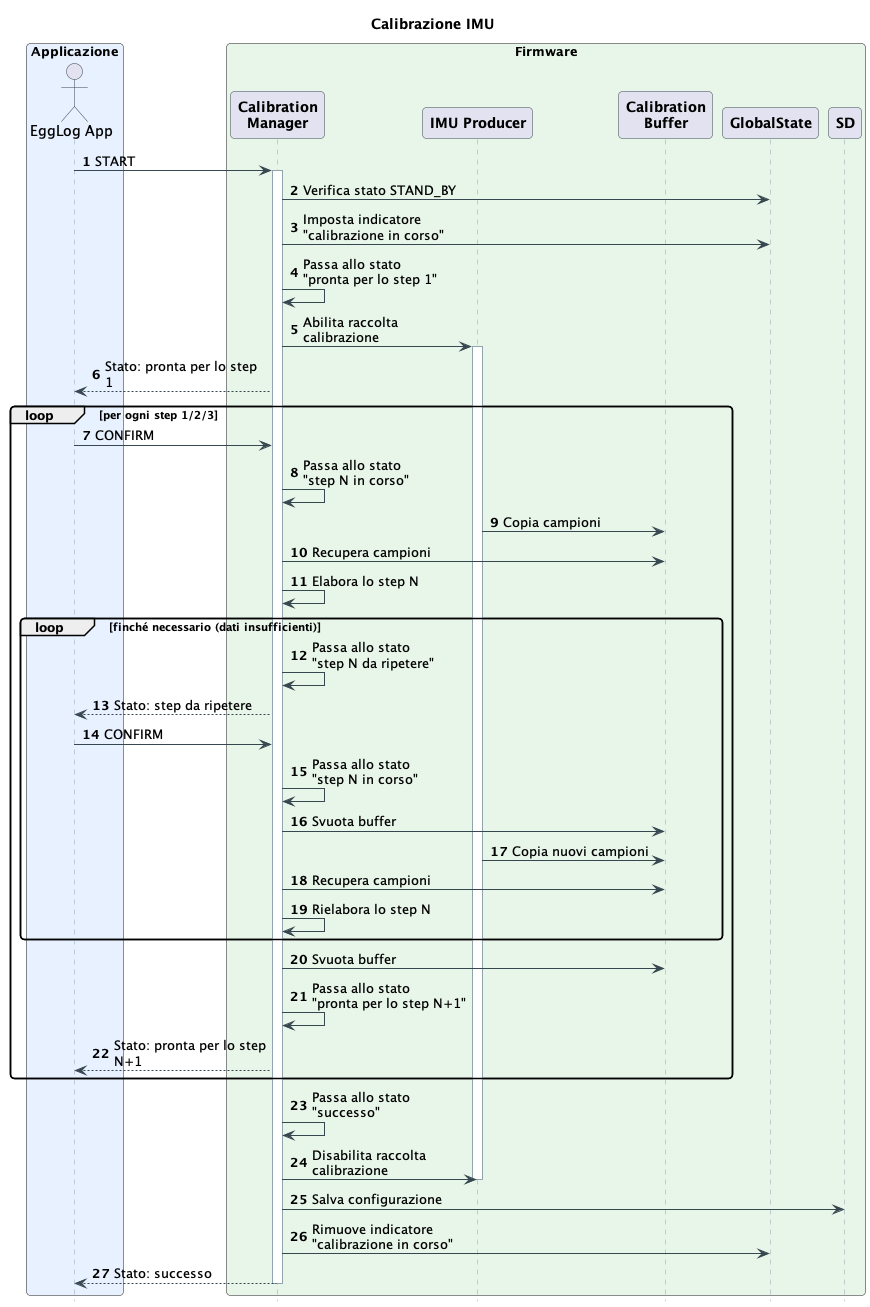
\includegraphics[width=1\textwidth]{../img/puml/diagrammi/Calibrazione-IMU.png}
    \caption{Diagramma della calibrazione dell'IMU}
\end{figure}

\newpage

\section{Valutazione tecnica sniffer CAN}

Durante il tirocinio è stata condotta una \textbf{valutazione tecnica} dell'interfacciamento di un nuovo microcontrollore con il bus CAN del motoveicolo, 
propedeutica alla realizzazione di un nodo \textit{sniffer} separato dal dispositivo EggLog principale. L'analisi ha riguardato sia l'aspetto \textbf{hardware}, 
relativo all'interfacciamento elettrico con il bus, sia l'aspetto \textbf{software}, relativo alla configurazione e alla gestione del controller CAN.

\subsection{Hardware}

Sono state valutate tre soluzioni hardware per l'interfacciamento elettrico con il bus, poste a confronto secondo un \textit{trade-off} tra \textbf{costo} e 
\textbf{rischio elettrico}, sia per il motoveicolo che per il microcontrollore.

\begin{table}[H]
    \centering
    \begin{tabular}{c p{8.5cm} c c}
        \hline
        \textbf{Opzione} & \textbf{Descrizione} & \textbf{Costo} & \textbf{Rischio} \\
        \hline
        1 & Controller CAN nativo integrato nel microcontrollore, con \gls{transceiver} 
        esterno e diodi (\gls{tvs}) in serie a protezione & Basso & Alto \\
        \hline
        2 & Modulo CAN esterno dedicato, con transceiver a 5V, collegato tramite un adattatore di livello logico 
        bidirezionale e dei diodi (TVS) in serie a protezione & Medio-Alto & Medio-Basso \\
        \hline
        3 & Transceiver CAN a \gls{isolamento-galvanico} completo & Alto & Basso \\
        \hline
    \end{tabular}

    \caption{Confronto tra le soluzioni considerate per l'interfacciamento CAN}
    \label{tab:confronto-can}
\end{table}

\subsubsection{Opzione 1 - protezione passiva}
Il controller CAN nativo del microcontrollore viene utilizzato con un transceiver esterno e dei diodi TVS dedicato alla soppressione 
dei \gls{transienti}, posto a protezione delle linee CAN in prossimità del connettore d'ingresso.

\subsubsection{Opzione 2 - modulo esterno con adattatore logico}

Impiego di un modulo CAN esterno con adattamento di livello logico bidirezionale. Questa opzione era stata inizialmente valutata nell'ottica di 
integrare la logica di traduzione CAN direttamente nel nodo centrale EggLog; tale scelta architetturale è stata tuttavia rivista nel corso della 
stessa valutazione tecnica, optando per un nodo sniffer separato e modulare, anche a causa dei limitati spazi disponibili sotto il codino della moto.

\subsubsection{Opzione 3 - isolamento galvanico completo}
Impiego di un transceiver CAN a isolamento galvanico integrato, sia di segnale sia di alimentazione, disponibile in commercio come componente singolo che integra 
isolatore digitale e convertitore di alimentazione isolato in un unico pacchetto. Elimina completamente il riferimento di massa comune tra il nodo sniffer e il veicolo, 
a fronte di costo e complessità di progettazione elettronica nettamente superiori.

\subsection{Scelta dell'Opzione 1 e schema elettrico del prototipo}

A completamento della valutazione tecnica delle tre soluzioni di interfacciamento (Tabella \ref{tab:confronto-can}), questa sezione approfondisce lo schema elettrico 
dell'\textbf{Opzione 1}, scelta per la realizzazione del prototipo. Tale soluzione è stata preferita in considerazione della natura ancora \textbf{esplorativa del progetto}, 
che ha reso prioritario disporre di un'architettura semplice e modulare, adeguata alla fase iniziale di sperimentazione. Lo schema viene quindi analizzato nel dettaglio, 
con particolare attenzione ai rischi elettrici individuati e alle relative mitigazioni adottate per renderli accettabili nel contesto del prototipo.

\subsubsection{Componenti dello schema}

EggLog CAN Sniffer è realizzato con i seguenti componenti:

\begin{itemize}
    \item \textbf{Microcontrollore}: ESP-WROOM-32, con controller CAN (\gls{twai}) nativo integrato;
    \item \textbf{Transceiver CAN}: modulo \textit{Waveshare SN65HVD230 CAN Board}\footcite{site:SN65HVD230}, alimentato a 3.3V. 
    Espone i pin: \texttt{VCC 3.3v} per l'alimentazione, \texttt{GND}, \texttt{CAN\_TX} e \texttt{CAN\_RX} 
    (come ingresso e uscita dati verso il microcontrollore), \texttt{CAN\_H} e \texttt{CAN\_L};
    \item \textbf{Protezione}: diodo TVS \textit{onsemi NUP2105LT1G}\footcite{site:NUP2105LT1G}, \textit{dual-channel}, posizionato in derivazione lungo le linee \texttt{CAN\_H} e
    \texttt{CAN\_L}, vicino al connettore diagnostico;
    \item \textbf{Massa}: collegamento a \texttt{Y} che parte dal \texttt{GND} dello shield CAN e arriva al \texttt{GND} della presa diagnostica della moto e
     il \texttt{GND} dell'ESP-WROOM-32.
\end{itemize}

Le linee dati verso il microcontrollore \texttt{CAN\_TX}/\texttt{CAN\_RX} restano a
livello 3.3V, direttamente compatibili con i GPIO dell'ESP-WROOM-32: non è quindi necessario alcun
adattatore di livello logico, a differenza di quanto previsto per l'Opzione 2 con modulo a 5V.

\subsubsection{Schema elettrico}

\begin{figure}[H]
    \centering
    \resizebox{\textwidth}{!}{%
    \begin{circuitikz}[
        x=0.85cm,
        y=0.85cm,
        font=\footnotesize,
        line width=0.8pt,
        american
    ]
        \node[
            draw, thick,
            rectangle,
            minimum width=2.7cm,
            minimum height=2.8cm,
            align=center,
            fill=blue!5
        ] (moto) at (0,3)
        {\textbf{Connettore}\\
         \textbf{diagnostico}\\
         \scriptsize (Yamaha)\\[1mm]
         \scriptsize GND\\
         \scriptsize CANH\\
         \scriptsize CANL\\
         \scriptsize\color{gray} 12\,V (non usato)};
 
        \node[
            draw, thick,
            rectangle,
            minimum width=2.6cm,
            minimum height=2.2cm,
            align=center,
            fill=orange!8
        ] (tvs) at (4.7,3)
        {\textbf{NUP2105L}\\[1mm]
         \small Protezione TVS};
 
        \node[
            draw, thick,
            rectangle,
            minimum width=3.2cm,
            minimum height=3.6cm,
            align=center,
            fill=green!8
        ] (shield) at (10.0,3)
        {\textbf{CAN Shield}\\
         \scriptsize (transceiver SN65HVD230)\\[2mm]
         \scriptsize CANH\,/\,CANL\\
         \scriptsize CAN\,TX\,/\,CAN\,RX\\
         \scriptsize GND\,/\,3.3\,V};

        \node[
            draw, thick,
            rectangle,
            minimum width=3.1cm,
            minimum height=3.6cm,
            align=center,
            fill=violet!8
        ] (esp) at (16.3,3)
        {\textbf{ESP-WROOM-32}\\[1mm]
         \small Controller TWAI\\[2mm]
         \scriptsize GND\,/\,3.3\,V\\
         \scriptsize GPIO 4\,/\,5};
 
        \draw[thick]
            ([yshift=0.5cm]moto.east) -- node[above] {\scriptsize CANH}
            ([yshift=0.5cm]tvs.west);
        \draw[thick]
            ([yshift=0.5cm]tvs.east) -- node[above] {\scriptsize CANH}
            ([yshift=0.5cm]shield.west);
 
        \draw[thick]
            ([yshift=-0.2cm]moto.east) -- node[below] {\scriptsize CANL}
            ([yshift=-0.2cm]tvs.west);
        \draw[thick]
            ([yshift=-0.2cm]tvs.east) -- node[below] {\scriptsize CANL}
            ([yshift=-0.2cm]shield.west);
 
        \draw[-Stealth, thick]
            ([yshift=1.35cm]esp.west) -- node[above] {\scriptsize 3.3\,V}
            ([yshift=1.35cm]shield.east);
 
        \draw[thick]
            ([yshift=0.45cm]esp.west) -- node[above] {\scriptsize CAN\,TX}
            ([yshift=0.45cm]shield.east);
 
        \draw[thick]
            ([yshift=-0.45cm]shield.east) -- node[below] {\scriptsize CAN\,RX}
            ([yshift=-0.45cm]esp.west);
 
        \draw[thick]
            (moto.south) -- (moto.south |- 0,-0.9);

        \draw[thick]
            (tvs.south) -- (tvs.south |- 0,-0.9);

        \draw[thick]
            (shield.south) -- (shield.south |- 0,-0.9);

        \draw[thick]
            (esp.south) -- (esp.south |- 0,-0.9);

        \draw[thick]
            (0,-0.9) -- (esp.south |- 0,-0.9);

        \node[ground] at (10.0,-0.9) {};

        \node[below, font=\scriptsize]
            at (7.3,0.0)
            {Massa comune (GND)};
 
    \end{circuitikz}%
    }
    \caption{Schema elettrico di EggLog CAN Sniffer.}
    \label{fig:schema-elettrico-sniffer}
\end{figure}

Lo schema evidenzia i tre punti chiave della soluzione adottata:

\begin{enumerate}
    \item il TVS \textbf{NUP2105L} è inserito \textit{in derivazione} su entrambe le linee \texttt{CAN\_H}/\texttt{CAN\_L}, il più vicino possibile
    all'ingresso, cosicché qualunque transiente proveniente dal bus moto venga limitato prima di raggiungere il transceiver dello shield;
    \item le linee digitali \texttt{TX}/\texttt{RX} tra shield ed ESP-WROOM-32 non richiedono protezione aggiuntiva né adattamento di livello, essendo
    lo shield già a 3.3V;
    \item la massa è condivisa tra moto, shield ed ESP-WROOM-32, poiché l'assenza di isolamento galvanico richiede un riferimento elettrico comune e 
    consente di mantenere le tensioni di modo comune delle linee CAN entro l'intervallo operativo del transceiver.
\end{enumerate}

Il prototipo è pensato per una \textbf{Yamaha MT-07}, la cui porta diagnostica è del tipo \textit{Sumitomo} a 4 pin: GND, 12v, \texttt{CAN\_H} e \texttt{CAN\_L}.
È stato quindi necessario prevedere l'aggiunta di un adattatore dedicato a tale connettore. 

Per estendere la compatibilità ad altri motoveicoli, uno sviluppo futuro prevede l'implementazione degli 
adattatori per i restanti formati più diffusi (3 pin, 6 pin e il connettore OBD standard).

\subsubsection{Analisi dei rischi}

Rispetto al confronto generale di Tabella \ref{tab:confronto-can}, il rischio elettrico più elevato dell'Opzione 1 deriva dall'assenza di
isolamento galvanico tra il nodo sniffer e il bus del veicolo: shield ed ESP-WROOM-32 condividono lo stesso riferimento di massa delle centraline
originali. I rischi specifici individuati e le relative mitigazioni sono riassunti di seguito. 

\begin{table}[H]
    \centering
    \begin{tabular}{p{4cm} p{6cm} p{4cm}}
        \hline
        \textbf{Rischio} & \textbf{Descrizione} & \textbf{Mitigazione} \\
        \hline
        Transienti sulle linee CAN & Scariche elettrostatiche o disturbi impulsivi del veicolo (accensione, bobine, motorino di
        avviamento) possono superare la tensione di breakdown dei pin del transceiver & TVS NUP2105L in serie: $V_{wm}=24$V,
        $V_{br}=26.2$V, $P_{ppm}=350$W/linea, $I_{ppm}=8$A \\
        \hline
        Interferenza con il bus del veicolo & Un nodo software difettoso potrebbe inviare ACK o frame di errore, disturbando la
        comunicazione tra le centraline & Controller TWAI configurato in modalità \texttt{listen-only}: nessun ACK né frame di
        errore attivo, indipendentemente da bug software \\
        \hline
        Riferimento di massa flottante & Se la massa dello shield non coincide con quella della moto, il transceiver può superare il
        proprio range di modo comune, causando errori di ricezione o stress sul componente & Collegamento di massa a Y tra moto,
        shield ed ESP-WROOM-32, sullo stesso nodo \\
        \hline
    \end{tabular}
    \caption{Rischi elettrici e relative mitigazioni}
\end{table}

La combinazione delle tre mitigazioni rende il rischio residuo coerente con l'obiettivo del prototipo, cioè verificare la fattibilità della 
soluzione minimale prima di eventualmente investire nelle Opzioni 2 o 3, che restano disponibili come evoluzione futura senza modifiche 
architetturali al resto del sistema.

\section{Architettura dello sniffer CAN}

\subsection{Architettura}

L'architettura software di EggLog CAN Sniffer è progettata secondo un'architettura \textbf{esagonale}, scelta motivata dal requisito
più delicato del sistema: gli identificativi dei frame CAN e le formule di decodifica variano da marca a marca, e spesso anche tra modelli diversi
dello stesso costruttore. Un'architettura a livelli tradizionale tenderebbe a concentrare questa conoscenza nel livello di logica applicativa
sotto forma di condizionali crescenti nel tempo.

Il dominio espone tre porte principali, ciascuna corrispondente a una responsabilità concettualmente indipendente:

\begin{itemize}
    \item una porta che astrae l'accesso al bus CAN fisico, implementata da un adattatore basato sul controller CAN in modalità ascolto passivo;
    \item una porta che astrae la decodifica specifica del veicolo, implementata da un adattatore dedicato per ciascun modello di veicolo supportato;
    \item una porta che astrae il canale di trasporto verso il nodo centrale, implementata da un adattatore basato su advertising BLE.
\end{itemize}

L'orchestrazione è affidata a un unico caso d'uso, che non conosce alcun dettaglio implementativo degli adattatori concreti, come illustrato in Figura~\ref{fig:c4-sniffer}.

\begin{figure}[H]
    \centering
    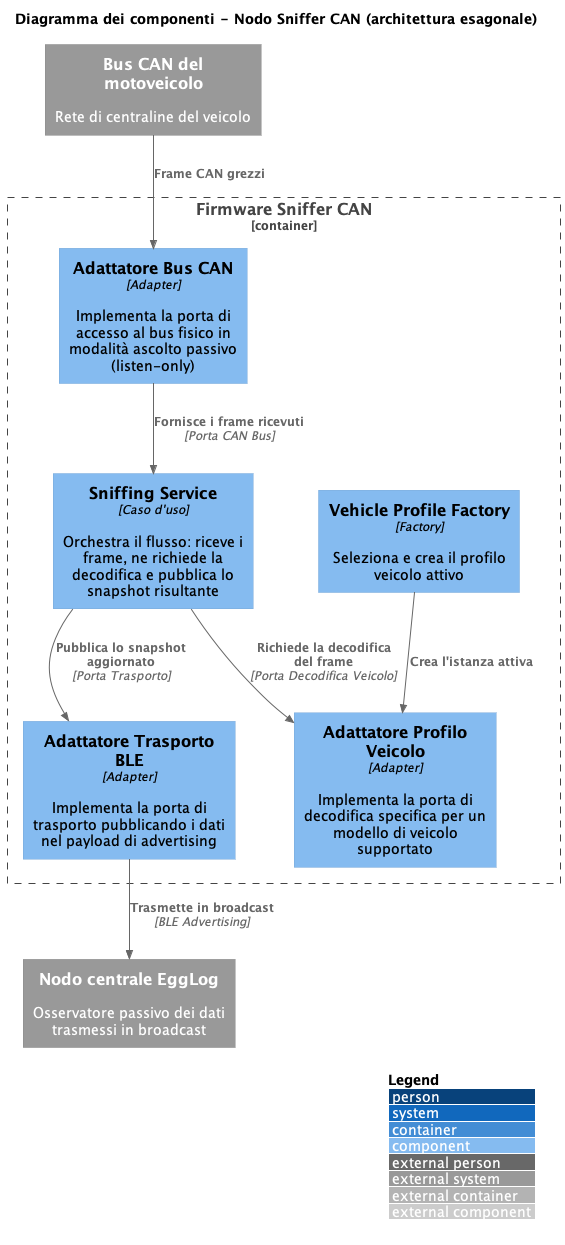
\includegraphics[width=0.6\textwidth]{../img/puml/c4/C4_Component_Sniffer.png}
    \caption{Diagramma dei componenti di EggLog CAN Sniffer: architettura esagonale}
    \label{fig:c4-sniffer}
\end{figure}

\subsection{Scelte progettuali}

\begin{itemize}
    \item \textbf{Strategy Pattern}: la conoscenza del veicolo è isolata dietro la porta di decodifica, di cui ogni modello supportato fornisce un
    adattatore concreto. \\
    \textit{Vantaggio}: la strategia di decodifica è selezionabile e sostituibile senza toccare dominio o logica applicativa,
    rendendo l'aggiunta di un nuovo veicolo un'estensione isolata anziché una modifica pervasiva.
    \item \textbf{Factory Pattern}: la selezione del profilo veicolo attivo è centralizzata in un unico punto di creazione. \\
    \textit{Vantaggio}:
    aggiungere il supporto a un nuovo modello richiede solo un nuovo adattatore e la relativa voce nel punto di creazione, senza modificare altre
    parti del firmware.
\end{itemize}

\begin{figure}[H]
    \centering
    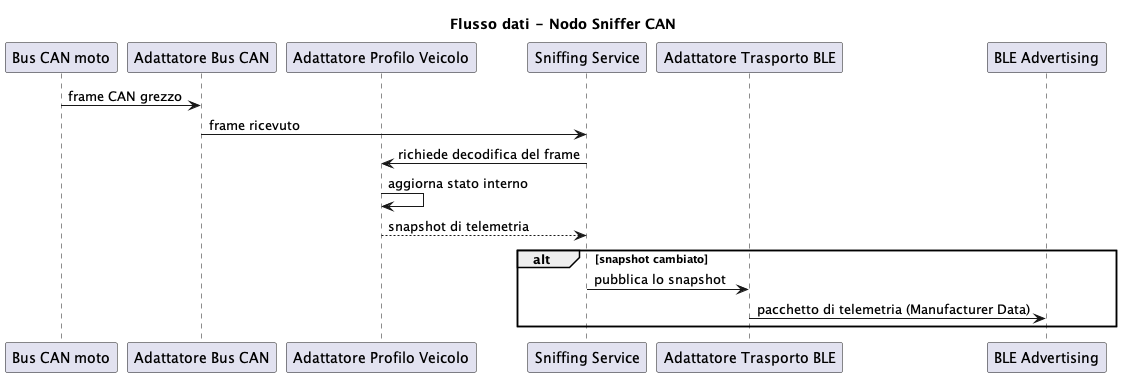
\includegraphics[width=\textwidth]{../img/puml/diagrammi/Dati-sniffer.png}
    \caption{Flusso dati dal bus CAN al payload BLE}
\end{figure}

\subsection{Trasporto dei dati: BLE advertising broadcast}

Il requisito di trasmissione continua e indipendente dalla presenza di un ricevitore attivo ha escluso l'uso di un canale BLE classico basato su
connessione con notifiche: senza un ricevitore connesso e sottoscritto, le notifiche non avrebbero alcun canale su cui viaggiare. La soluzione
adottata sfrutta invece il payload di \textbf{advertising} BLE: EggLog CAN Sniffer non espone alcun servizio dedicato e non accetta connessioni,
trasmettendo i dati all'interno del pacchetto di advertising stesso. 
Il nodo centrale EggLog agisce da semplice osservatore
passivo, leggendo il payload durante le proprie scansioni senza mai stabilire una connessione: un modello \emph{publish-only}, tollerante alle
perdite, coerente con un flusso di telemetria senza garanzie di consegna per il singolo campione.

Il pacchetto trasmesso include la versione del protocollo, il profilo veicolo attivo, marcia, apertura farfalla, RPM, velocità, temperature motore
e aria, e un contatore progressivo per rilevare pacchetti persi o duplicati.

\begin{figure}[H]
    \centering
    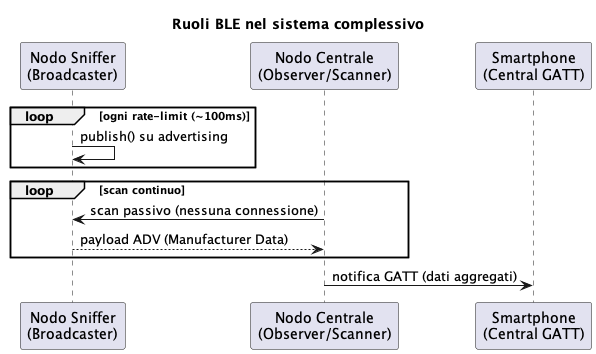
\includegraphics[width=0.7\textwidth]{../img/puml/diagrammi/Ruolo-BLE-generale.png}
    \caption{I tre ruoli BLE nel sistema complessivo}
\end{figure}


\chapter{Implementazione}

\textit{In questo capitolo viene descritto il lavoro di implementazione svolto, mostrando come le scelte progettuali illustrate nel capitolo precedente
si sono tradotte in codice effettivo.}

\newpage